% !TeX program = lualatex
\documentclass[11pt]{beamer}
\usefonttheme[onlymath]{serif}
\usepackage[utf8]{inputenc}
\usepackage[T1]{fontenc}
\usepackage{bbm}
\usepackage{lmodern}
% \usepackage[hidelinks]{hyperref}
\usepackage[autolanguage]{numprint}
\usepackage[french]{babel}
\usepackage{graphicx}
    \graphicspath{{./fig/}}
\usepackage{listings}


\usepackage{fontawesome} %font fa logo

\usepackage{color}
\definecolor{dkgreen}{rgb}{0,0.6,0}
\definecolor{gray}{rgb}{0.5,0.5,0.5}
\definecolor{mauve}{rgb}{0.58,0,0.82}

\lstset{ %
	language=R,                     % the language of the code
	basicstyle=\footnotesize,       % the size of the fonts that are used for the code
	numbers=left,                   % where to put the line-numbers
	numberstyle=\tiny\color{gray},  % the style that is used for the line-numbers
	stepnumber=1,                   % the step between two line-numbers. If it's 1, each line
	% will be numbered
	numbersep=5pt,                  % how far the line-numbers are from the code
	showspaces=false,               % show spaces adding particular underscores
	showstringspaces=false,         % underline spaces within strings
	showtabs=false,                 % show tabs within strings adding particular underscores
	tabsize=4,                      % sets default tabsize to 2 spaces
	captionpos=b,                   % sets the caption-position to bottom
	%breaklines=true,                % sets automatic line breaking
	breakatwhitespace=false,        % sets if automatic breaks should only happen at whitespace
	title=\lstname,                 % show the filename of files included with \lstinputlisting;
	% also try caption instead of title
	keywordstyle=\color{blue},      % keyword style
	commentstyle=\color{mauve},   % comment style
	stringstyle=\color{dkgreen},      % string literal style
	escapeinside={\%*}{*)},         % if you want to add a comment within your code
	morekeywords={*,...}            % if you want to add more keywords to the set
}

  %% Renvois vers les scripts R
  %%%%% Update color if name change
\newcommand{\gotoR}[1]{%
	\begin{center}
		\colorbox{ulgold}{\color{black}
			\makebox[75mm][c]{%
				\makebox[5mm]{\raisebox{-1pt}{\large\faChevronCircleDown}}\;%
				{\ttfamily #1}}}
\end{center}}


\hypersetup{
  colorlinks=true,
  citecolor=blue,
  linkcolor=black,
  filecolor=magenta,
  urlcolor=cyan,
}

\mode<presentation> {
  % \useoutertheme{infolines} % Pour les thèmes qui n'ont pas de pied-de-page
  \usetheme{ulaval}
  %\usecolortheme{ulaval}
  % \setbeamercovered{transparent}
  \setbeamercovered{invisible}
}


\logo{%\includegraphics[height=0.6cm]{COPL}\hspace{.5cm}%

\includegraphics[height=1.5cm]{DotLayer_logo_short_COL_RVB}}%\hspace{.2cm}\vspace{.865\paperheight}}
\titlegraphic{
	
\includegraphics[height=1cm]{DotLayer_logo_full+tagline_COL_RVB}\vspace{0.7cm}
	
\includegraphics[height=1cm]{logo-universite-laval}\vspace{0.7cm}
	
\includegraphics[height=1cm]{crdm}\vspace{0.7cm}
	
\includegraphics[height=1cm]{graal}\vspace{0.7cm}
}

\title[Les tests automatis\'es en R]{Les tests automatis\'es en R}
%\subtitle[]{}

\subtitle{Comment maintenir son code}

\author[D. Beauchemin \& C. Blier-Wong]{David Beauchemin, BSc. et \\ Christopher Blier-Wong, MSc.}
\institute[.Layer]
{
	.Layer, Université Laval, CRDM, GRAAL
}
\date{14 mai 2019, R à Québec 2019}

\AtBeginSection[]
  {
     \begin{frame}<beamer>
     \frametitle{Agenda}
     \tableofcontents[currentsection]
     \end{frame}
  }

  \newenvironment{slide}[1]
{\begin{frame}[environment=slide]
\frametitle{\insertsection \newline \large{#1}}}
{\end{frame}}

\usepackage{fontspec}

\setsansfont[Path=Muli/, BoldFont=Muli-Bold.ttf,
ItalicFont=Muli-Italic.ttf,
BoldItalicFont=Muli-BoldItalic.ttf]{Muli-Regular.ttf}%



\begin{document}

\begin{frame}[label=titre, plain]
\titlepage
\end{frame}

\section[Introduction]{Introduction}

\begin{frame}{Qui nous sommes}
\begin{itemize}
	\item Étudiants avec intérêt commun à l'actuariat, l'informatique et l'intelligence artificielle
	\item Membres de .Layer, une communauté ayant comme mission de promouvoir la collaboration et le partage de connaissances dans le domaine de la science des données.
	\item Organisateurs de conférences, ateliers et autres événements.
\end{itemize}
\begin{center}
	\href{dotlayer.org}{dotlayer.org}\\
	
\includegraphics[height = 0.3cm]{facebook} : \href{https://www.facebook.com/MeetupMLQuebec/}{MeetupMLQuebec}
\end{center}
\end{frame}

\begin{frame}{Quelques considérations}
\begin{itemize}
\item Quand on dit "les autres" dans cette présentation, ça veut aussi dire vous dans le futur !
\item Il y a différentes philosophies de test pour chaque paradigme de programmation. Dans cet atelier, on considère le \textsf{R} comme un langage procédural contrairement à fonctionnel
\end{itemize}
\end{frame}

\begin{frame}{Quelques considérations}

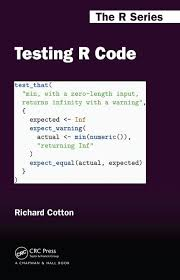
\includegraphics[height=0.25\textheight]{testingRcode} \hfill
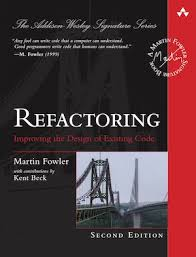
\includegraphics[height=0.25\textheight]{refactoring} \hfill
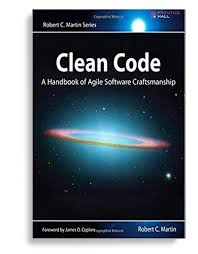
\includegraphics[height=0.25\textheight]{cleanCode} \hfill
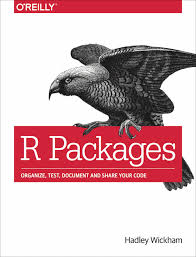
\includegraphics[height=0.25\textheight]{packages} \hfill
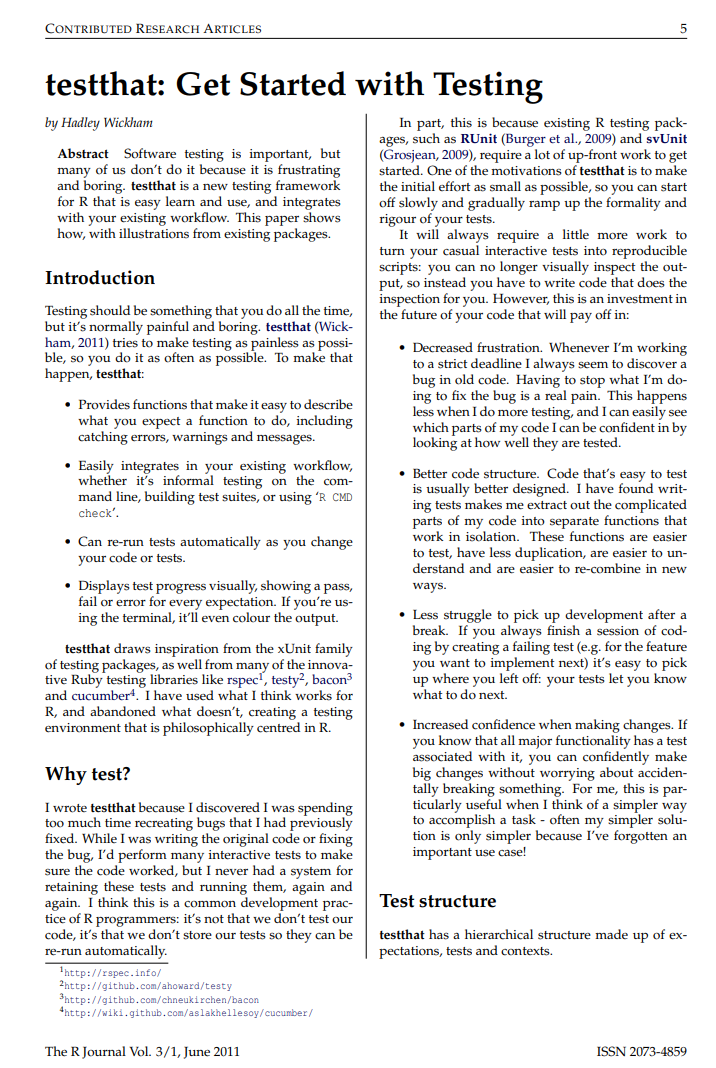
\includegraphics[height=0.25\textheight]{testthat}

\end{frame}

\begin{frame}{Le \textit{clean code}}
\begin{itemize}
    \item Le test unitaire est une pratique du \textit{clean code}
    \item Le \textit{clean code} est une pratique de génie informatique qui dicte que le code doit être propre.
\end{itemize}
\begin{block}{}
{\large ``Any fool can write code that a computer can understand. Good programmers
write code that \textbf{humans} can understand.''}
\vskip5mm
\hspace*\fill{\small--- Martin Fowler}
\end{block}
\end{frame}

\begin{frame}{Le \textit{clean code}}
\textit{Mais quand on compile, ça n'a pas d'importance si le code est propre}

Un code propre permet de collaborer facilement et de réduire les bogues.
\begin{itemize}
    \item Quand on écrit du code, on sait (dans notre tête) ce que les variables représentent.
    \item Ward Cunningham (fondateur, wiki) : on doit passer cette compréhension de la tête au code lui-même.
    \item Pour que les autres comprennent ce que vous faites sans avoir à lire les assignations.
\end{itemize}
\end{frame}

\begin{frame}{Les tests pour les scientifiques des données}
En \textsf{R}, les principales tâches sont :
\begin{itemize}
\item D'interagir avec des données afin de calculer des statistiques ou de l'information intéressante (exploration)
\item D'automatiser ces tâches d'exploration sur plusieurs jeux de données ou sur plusieurs tâches (programmation)
\item De rassembler un ensemble de fonctions et publier un paquetage pour partager aux autres (partage)
\end{itemize}
\end{frame}

\begin{frame}{Les tests pour les scientifiques des données}
\framesubtitle{Exploration}
Les tests ne sont pas nécessaires si les tâches d'exploration
\begin{itemize}
	\item comptent quelques lignes seulement;
	\item sont simples;
	\item font seulement appel à des fonctions prédéfinies.
\end{itemize}
\end{frame}

\begin{frame}{Les tests pour les scientifiques des données}
\framesubtitle{Programmation}
On désire des tests dans les tâches de programmation pour
\begin{itemize}
\item s'assurer que notre fonction a le comportement voulu
\item s'assurer qu'on ne brise pas quelque chose qui fonctionnait dans le passé
\item avoir une documentation qui défini les comportements
\end{itemize}
Les tests pendant la programmation servent à vérifier que le programmeur n'a pas fait d'erreur.
\end{frame}

\begin{frame}{Les tests pour les scientifiques des données}
\framesubtitle{Partage}
On désire des tests dans les tâches de partage pour
\begin{itemize}
\item s'assurer que les utilisateurs respectent les conditions d'utilisation de votre fonction.
\item important quand on publie des paquetages.
\end{itemize}
Les tests pendant le partage servent à vérifier que l'utilisateur n'ai pas fait d'erreur
\end{frame}

\begin{frame}{Deux principales philosophies de tests}

Le \textsf{R} compte deux grandes philosophies de tests.

\begin{itemize}
\item Les tests pour s'aider
\item Les tests pour aider les autres
\begin{block}{}
{\large ``The point of development-time testing is to make sure that you
haven’t done something stupid. By contrast, the point of run-time
testing is to make sure that the user hasn’t done something stupid.''}
\vskip5mm
\hspace*\fill{\small--- Richard Cotton}
\end{block}

\end{itemize}
\end{frame}

\begin{frame}{Deux principales philosophies de tests}
\framesubtitle{Les tests pour s'aider}
Les tests lors du développement
\begin{itemize}
\item Ils incluent les tests unitaires
\item On isole chaque partie d'un programme en fonctions
\item On valide que le comportement de chaque fonction est bon
\item On exécute les tests pour s'assurer qu'on n'a pas introduit de bogues
\item C'est très simple avec testthat
\item C'est l'objectif de l'atelier
\end{itemize}
\end{frame}

\begin{frame}{Deux principales philosophies de tests}
\framesubtitle{Les tests pour aider les autres}
Les tests lors du partage
\begin{itemize}
\item Quand on écrit une fonction, on a une utilité en tête
\item D'autres personnes vont peut-être vouloir l'utiliser pour une tâche différente : les gens sont créatifs !
\item Paquetage assertive.
\end{itemize}
\end{frame}

\begin{frame}{Qu'est-ce qu'un test unitaire ?}
\begin{itemize}
	\item Comme dans un examen, on souhaite valider le résultat d'un calcul
	\item Souvent, on teste le comportement d'une seule fonction
	\item Exemples : 
	\begin{itemize}
		\item valider que \texttt{somme(1, 1) == 2}
		\item valider que \texttt{somme("a", "b")} retourne une erreur
		\item valider qu'une fonction qui calcule un pourcentage retourne une valeur entre 0 et 100
		\item valider qu'une fonction qui calcule une proportion retourne une valeur entre 0 et 1
		\item valider que la valeur maximale d'un pourcentage est 100 et que la valeur maximale d'une proportion est 1
	\end{itemize}
\end{itemize}
\end{frame}


\begin{frame}{Quand dois-je écrire mon test ?}
À quel moment est-ce que le test devrait être écrit ?
\begin{enumerate}
\item Après avoir écrit un script
\item Avant d'avoir écrit la fonction
\end{enumerate}
\end{frame}

\begin{frame}{Quand est-ce que je dois écrire mon test ?}
\framesubtitle{Situation 1}
On considère la situation suivante :
\begin{enumerate}
\item On définit une tâche
\item On se donne des paramètres jouets
\item On construit un script pour donner la réponse attendue
\item On extrait une fonction du script
\item On efface le script
\end{enumerate}
On perd une information importante : une condition que la fonction doit respecter !
\end{frame}

\begin{frame}{Quand est-ce que je dois écrire mon test ?}
\framesubtitle{Situation 1}
À la place, on
\begin{enumerate}
\item Conserve le résultat attendu dans un test
\item C'est le cas le plus facile, on a déjà tous les ingrédients !
\end{enumerate}
\end{frame}

\begin{frame}{Quand est-ce que je dois écrire mon test ?}
\framesubtitle{Situation 2}
On considère la situation suivante :
\begin{enumerate}
\item On regarde un script qu'on a fait il y a longtemps
\item On veut utiliser le code dans une autre tâche
\end{enumerate}
\end{frame}

\begin{frame}{Quand est-ce que je dois écrire mon test ?}
\framesubtitle{Situation 2}
Alors, on
\begin{enumerate}
\item On se définit des conditions que la fonction doit respecter (tests)
\item On écrit la fonction de telle sorte que les tests passent
\end{enumerate}
On s'assure de ne rien briser !
\end{frame}

\begin{frame}{Quand est-ce que je dois écrire mon test ?}
\framesubtitle{Situation 3}
On considère la situation suivante :
\begin{enumerate}
\item On regarde une fonction
\item Elle contient plusieurs comportements, cas et conditions
\item On désire ajouter un comportement
\end{enumerate}
La fonction est possiblement utilisée à d'autres endroits, il ne faut pas changer ce qu'elle fait, seulement comment elle le fait.
\end{frame}

\begin{frame}{Quand est-ce que je dois écrire mon test ?}
\framesubtitle{Situation 3}
Alors, on
\begin{enumerate}
\item Écrit des tests pour valider le comportement du code total
\item On extrait des fonctions individuelles pour chaque comportement, cas et conditions
\item On exécute les tests à chaque changement
\end{enumerate}
\end{frame}

\begin{frame}{Quand est-ce que je dois écrire mon test ?}
\framesubtitle{Après avoir écrit un script}
Situation 3 : quand on a mal programmé
\begin{block}{}
Fail fast, fail often
\end{block}
\begin{itemize}
\item Plus on teste souvent, plus il est facile de diagnostiquer le problème
\item C'est facile, faire des erreurs.
\end{itemize}
\end{frame}

\section[Un premier test unitaire]{Un premier test unitaire}

\begin{frame}{Un premier test unitaire}
\framesubtitle{Le compromis complexité-rapidité}
Faire des exemples de tests dans un atelier est difficile.
\begin{itemize}
\item Si les programmes valent la peine de faire des tests, ils sont trop longs à expliquer.
\item Si les programmes sont trop simples, ça ne vaut pas la peine de faire tests.
\end{itemize}

Tester son code est simple. La difficulté est développer de l'habitude.
\end{frame}

\begin{frame}{Un premier test unitaire}
Avant d'utiliser \textit{testthat}, on écrit notre propre test à la main.

\begin{block}{La moyenne géométrique}
\gotoR{Exercices/partie\_1/exercices\_1.R}
\begin{equation*}
\left(\prod_{i = 1}^{n}x_i\right)^{\frac{1}{n}}  =
(-1)^m \exp\left(\frac{1}{n}\sum_{i = 1}^{n}\ln |x_i|\right)
\end{equation*}
\centering Où $m$ est le nombre de valeurs négatives dans le vecteur $x$.
\end{block}
\end{frame}


\section[Le paquetage \emph{testthat}]{Le paquetage \emph{testthat}}

\subsection[Introduction \`a l'interface de \emph{testthat}]{Introduction \`a l'interface de testthat}
\begin{frame}{L'interface générale d'un test \emph{testthat}}
Un test \textit{testthat} se divise en deux parties:
\begin{itemize}
	\item Le nom du comportement testé %(\textit{desc})
	\item Le code du test qui se sous-divise en deux parties: %(\textit{code}):
	\begin{itemize}
		\item  La valeur retournée par le comportement testé (\textit{optionnel selon la situation})
		\item L'évaluation du comportement testé
	\end{itemize}
\end{itemize}
\end{frame}

\begin{frame}{Exemple \textit{testthat}}
\begin{block}{Scénario: Calculer une valeur logarithmique}
Une valeur positive, \\
application de la transformation logarithmique naturelle, \\
retourne la valeur transformée.
\end{block}
\end{frame}

\begin{frame}[fragile]{Exemple \textit{testthat}}
\begin{block}{Scénario: Calculer une valeur logarithmique}
\begin{lstlisting}
UNE_VALEUR_POSITIVE <- 1
VALEUR_ATTENDUE <- 0

test_that("Une valeur positive,
            transformation ln,
            valeur ln adéquate.",{
        actual <- log(UNE_VALEUR_POSITIVE)
        expect_equal(expected = VALEUR_ATTENDUE, actual, 
        		tolerance=1e-8)})
\end{lstlisting}
\end{block}
% rajouter explication sur clarté de expected et actual!
\end{frame}

\begin{frame}{Exercices \textit{testthat}}
\begin{block}{Scénario: Moyenne géométrique}
\gotoR{Exercices/partie\_1/exercices\_2.R}
\end{block}
\end{frame}

\subsection[\emph{testthat} en d\'etails]{\emph{testthat} en d\'etails}

\begin{frame}{Le workflow \textit{testthat}}
Rappel : un test avec \textit{testthat} est composé

\begin{enumerate}
\item d'un entête en caractères pour décrire le test
\item du test, qui est composé
\begin{enumerate}
\item d'un appel à une fonction;
\item d'un résultat désiré;
\item d'une comparaison entre l'appel et le résultat.
\end{enumerate}
\end{enumerate}
\end{frame}

\begin{frame}{Les tests automatisés en R}
\begin{itemize}
\item Exécuter les tests doit être facile et rapide.
\item On doit pouvoir exécuter tous les tests quand on applique un changement.
\item testthat facilite cette tâche, mais on doit suivre un schéma particulier.
\end{itemize}
\end{frame}

\begin{frame}{La structure de tests}
\framesubtitle{La structure de fichiers}
\begin{itemize}
\item Placer tous les fichiers de test dans un répertoire
\item Un fichier de tests contient plusieurs tests
\item Les tests sont organisés par hiérarchie :
\begin{itemize}
    \item les résultats attendus sont regroupés dans les tests
    \item les tests sont regroupés dans des fichiers
    \item les fichiers sont regroupés dans des répertoires.
\end{itemize}
\end{itemize}
\end{frame}

\begin{frame}{Les tests automatisés en R}
\begin{itemize}
\item Un résultat attendu décrit le résultat d'un calcul. Il vérifie que le comportement est approprié.
\item Un test regroupe plusieurs résultats attendus pour une seule fonction / une seule fonctionnalité. C'est parfois appelé un test unitaire.
\item Un fichier regroupe plusieurs tests similaires ou reliés.
\end{itemize}
\end{frame}

\begin{frame}{Les résultats attendus}
\begin{itemize}
\item Un résultat attendu est le plus petit niveau de test.
\item Il commence par \texttt{expect\_}
\item Il contient deux arguments : le résultat actuel, et le résultat attendu
\item Les deux arguments doivent correspondre.
\end{itemize}
\end{frame}

\begin{frame}{Les résultats attendus}
\framesubtitle{Les \emph{expect\_}}
\begin{itemize}
\item \texttt{expect\_equal}
\item \texttt{expect\_identical}
\item \texttt{expect\_match}
\item \texttt{expect\_output}
\item \texttt{expect\_error}
\item \texttt{expect\_warning}
\item \texttt{expect\_true}, \texttt{expect\_false} et \texttt{expect\_null}
\item \texttt{ls("package:testthat", pattern = "\^{}expect")}
\end{itemize}
\end{frame}

\begin{frame}{Les tests}
\begin{itemize}
\item Chaque test doit avoir un nom informatif qui explique ce qui se passe
\item Quand le test échoue, c'est un des messages qui est affiché
\item Le message doit permettre d'identifier l'erreur rapidement
\item Pensez : Tester que : donné ..., quand ..., alors ...
\end{itemize}
\end{frame}

\begin{frame}{Les tests}
\begin{itemize}
\item On définit un nouveau test avec test\_that
\item Un test devrait tester un comportement
\item Il peut avoir plusieurs résultats attendus dans un test
\end{itemize}
\end{frame}

\begin{frame}{Exécuter les tests}
\begin{itemize}
\item {\texttt{test\_file}} exécute tous les tests dans un fichier
\item {\texttt{test\_dir}} exécute tous les fichiers dans un répertoire
\item \texttt{test\_check} si vous développez des paquetages
\end{itemize}
\end{frame}

\begin{frame}{Exécuter les tests}
\framesubtitle{Changer les rapports}
\begin{itemize}
\item \texttt{test\_file("test-file.R", reporter = "summary")}
\item \texttt{"minimal"} : une ligne
\item \texttt{"stop"} : arrêt à l'échec
\item \texttt{"silent"} : aucun, mais retourne une
\item \texttt{"rstudio"} : Entre summary et minimal : une ligne par échec
\item \texttt{"tap"} : "Test Anything Protocol"
\item \texttt{"check"} : Pour les paquetages
\end{itemize}
\end{frame}

\begin{frame}{Organisation des tests}
\framesubtitle{Les contextes}
\begin{itemize}
\item On peut avoir un fichier par test
\item On peut avoir un fichier avec tous les tests
\item On cherche un compromis
\item On peut diviser un fichier en contextes.
\end{itemize}
\end{frame}

\begin{frame}{Quoi tester}
\begin{block}{}
Quand vous êtes tentés d'écrire quelque chose avec un \textit{print}, écrire un test à la place. -- Martin Fowler
\end{block}
\begin{itemize}
\item Comportements attendus
\item Exemples négatifs
\item Erreurs attendues
\end{itemize}
\end{frame}

\begin{frame}{Plus d'information sur les tests}
\begin{itemize}
\item Quelle valeur a fait échouer la fonction ?
\item Quelle itération de la boucle a échoué ?
\end{itemize}
\end{frame}

\section[\'Ecrire du code testable : conseils et d\'eveloppement conduit par tests]{\'Ecrire du code testable : conseils et d\'eveloppement conduit par tests}

\begin{frame}{Bien écrire nos tests}
Un test se divise en trois parties:
\begin{itemize}
	\item Étant donné (\textit{given})
	\item Quand (\textit{when})
	\item Alors (\textit{then})
\end{itemize}
Cette segmentation permet une approche par exemple de comportement.
% On doit pouvoir lire les parties comme du texte d'un livre

% Source https://www.martinfowler.com/bliki/GivenWhenThen.html
\end{frame}

\begin{frame}{\textit{Given}}
Il s'agit de notre état avant le début du comportement du scénario que l'on teste. (précondition)

\begin{block}{Scénario: Calculer une valeur logarithmique}
\textit{\textbf{Given}} Une valeur positive.
\end{block}
\end{frame}

\begin{frame}{\textit{When}}
Il s'agit du comportement à tester de notre scénario que l'on teste. (\emph{LE} test)

\begin{block}{Scénario: Calculer une valeur logarithmique}
\textit{\textbf{When}} Application de la transformation logarithmique naturelle.
\end{block}
\end{frame}

\begin{frame}{\textit{Then}}
Il s'agit de la résultante de la transformation sur notre état initial.
\begin{block}{Scénario: Calculer une valeur logarithmique}
\textit{\textbf{Then}} Retourne la valeur transformée.
\end{block}
\end{frame}

\begin{frame}[fragile]{Exemple \textit{testthat}}
\begin{block}{Scénario: Calculer une valeur logarithmique}
	\begin{lstlisting}
	UNE_VALEUR_POSITIVE <- 1
	VALEUR_ATTENDUE <- 0
	
	test_that("Une valeur positive,
	transformation ln,
	valeur ln adéquate.",{
	actual <- log(UNE_VALEUR_POSITIVE)
	expect_equal(expected = VALEUR_ATTENDUE, actual, 
	tolerance=1e-8)})
	\end{lstlisting}
\end{block}
% rajouter explication sur clarté de expected et actual!
\end{frame}

\begin{frame}{Bien utiliser nos tests}
\begin{itemize}
\item Documentation par comportement.
\item Facilite la lisibilité.
\item Meilleure confiance lors d'intégration des composantes dans une architecture plus complexe.
\item Rapidité de développement.
\end{itemize}
\end{frame}

\begin{frame}{\textit{Testability}}
\begin{block}{}
{\large ``Ideally, development-time tests should be written once and run lots of times.''}
\vskip5mm
\hspace*\fill{\small--- Richard Cotton}
\end{block}
\end{frame}

\begin{frame}{\textit{Testability}}
Que peut-on \textit{faire} avec la \textit{testability}
\begin{itemize}
	\item Ajouter des fonctionnalités rapidement.
	\item Pouvoir partager son code avec confiance.
	\item Créer un paquetage et contribuer à la collectivité R.
	\item Ne pas être obligé de \textit{jeter} son code.
\end{itemize}
\end{frame}

\begin{frame}{\textit{Tell don't ask} en R}

Laisser la propriété des données aux objets propriétaire.

\begin{block}{}
{\large ``[...] rather than asking an object for data and acting on that data, we should instead tell an object what to do. This encourages to move behavior into an object to go with the data.''}
\vskip5mm
\hspace*\fill{\small--- Martin Fowler}
\end{block}
\end{frame}

\begin{frame}[fragile]{\textit{Tell don't ask} en R}
\begin{block}{Dire quoi faire aux données}
\begin{lstlisting}
mean(data[data > median(data)])

moyenne_valeurs_supp_medianne(data)
\end{lstlisting}
\end{block}
\end{frame}

\begin{frame}{\textit{Refactoring}}
\begin{block}{}
{\large ``A change made to the internal structure of [your code] to make it easier to understand and cheaper to modify without changing its observable behavior.''}
\vskip5mm
\hspace*\fill{\small--- Martin Fowler}
\end{block}
\end{frame}

\begin{frame}[fragile]{\textit{Refactoring}}
\begin{block}{}
\begin{lstlisting}
mean(data[data > median(data)])

moyenne_valeurs_supp_medianne(data)
\end{lstlisting}
\end{block}

Il s'agit d'un processus en continu!
\end{frame}




\begin{frame}{Exercices}
\begin{block}{\textit{Refactoring} de code}
À partir du code fourni en échange, effectuer du \textit{refactoring} pour sortir les fonctions préalablement définies sans toucher aux tests.
\end{block}

\begin{block}{Ajout d'une fonctionnalité}
À partir du code de l'exercice de \textit{refactoring}, ajoutez la fonctionnalité qui calcule le ratio de la moyenne des moyennes sur la variance des moyennes. Écrire les tests en conséquence.
\end{block}
\end{frame}

%20 mins exercices
\begin{frame}{\textit{Boy scout rule}}

Nous sommes mutuellement responsables de la qualité du code.

\begin{block}{}
{\large ``Always leave the code you're editing a little better than you found it.''}
\vskip5mm
\hspace*\fill{\small--- Robert C. Martin}
\end{block}
\end{frame}

%10 min buffer

\begin{frame}{Conclusion}
\begin{itemize}
	\item Les tests automatisés en R sont beaucoup plus faciles avec \textit{testthat}.
	\item Les tests sont importants pour améliorer le développement de votre code informatique.
\end{itemize}

\begin{block}{}
\centering Assurance qualité, R et calcul scientifique, demain @ 13:55 
\end{block}
\end{frame}

\end{document}
